\chapter{\uppercase{Future Work and Preliminary Results} \label{chapter:future}}


\section{Alternative Experimental Designs}

In this section we return to the nonlinear examples presented in the previous chapter and address the choices made in experimental design.
We demonstrate that the decisions made regarding measurement equipment and/or location have an impact on the reduction of uncertainty and accuracy of the MUD point.

We demonstrate the use of the WME map defined in \eqref{eq:qoi_WME_fixed_data} on a problem incorporating a single stream of time-series data for a first-order ODE problem.

\subsection{ODE Example}
Consider an exponential decay problem with uncertain decay rate:

$$
\begin{cases}
\frac{\partial u}{\partial t} & = \param u(t) \\ u(0) &= 0.75
\end{cases}
$$

The solution is described by
\begin{equation}
  u(t) = u_0\exp(-\param t), \; u_0 = 0.75 ,
\end{equation}
where we consider $t \in [0, 3]$, allowing measurements to begin for $t\geq 1$.
\begin{figure}[htbp]
  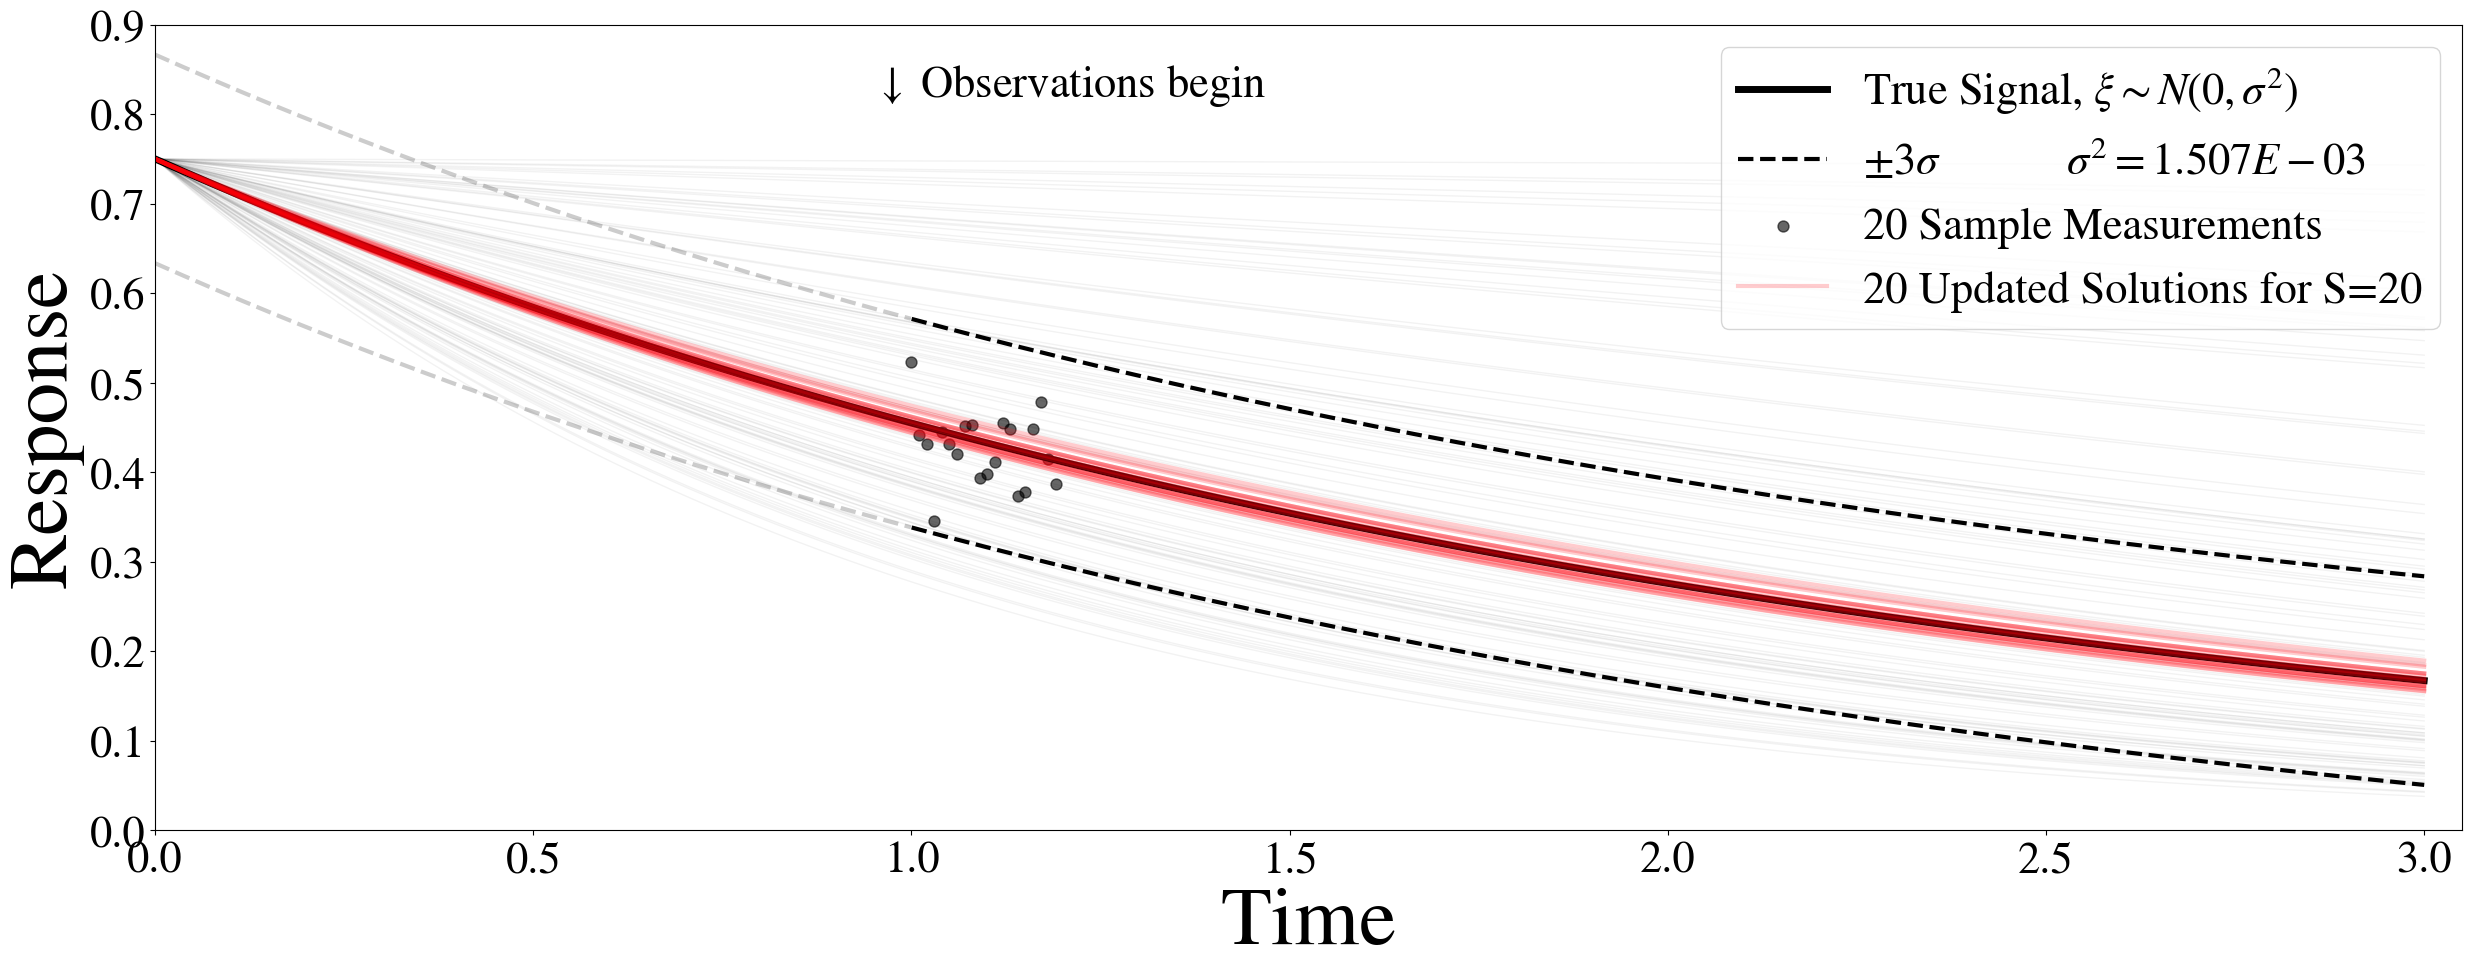
\includegraphics[width=\linewidth]{figures/ode/ode_20_reference_solution}
  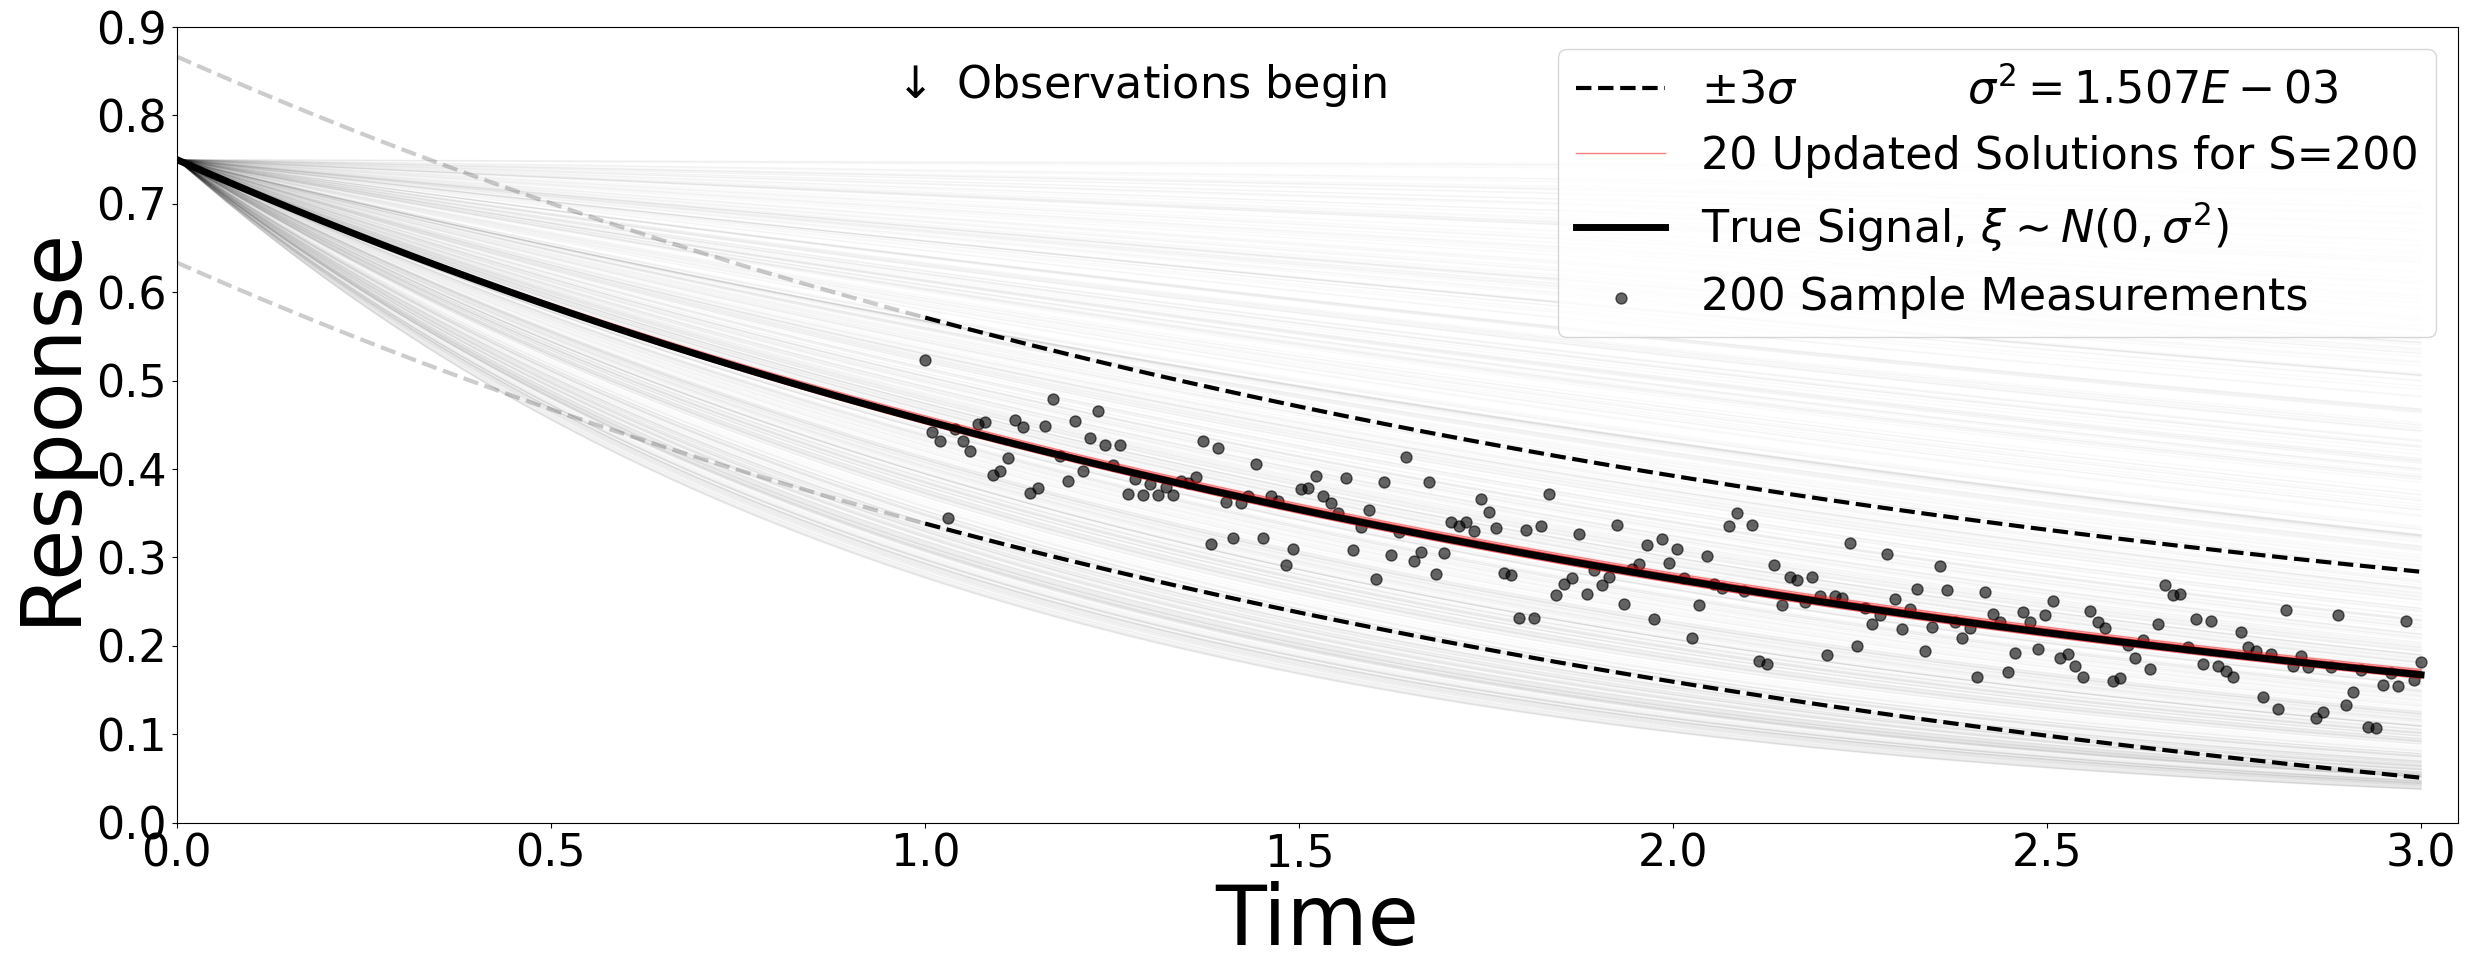
\includegraphics[width=\linewidth]{figures/ode/ode_200_reference_solution}
  \caption{Time series response for exponential decay with markers for the assumed error intervals for observations.
  Measurements are taken over the time interval $(1,3)$.
  Five-hundred draws from $\pi_\text{init}$ are used to generate sample responses and are shown in gray.
  (Top): Twenty updated solution (the results of the repeated trials) for $S=25$ are plotted in blue, and capture the true signal.
  (Bottom): The solution for using all $S=200$ measurements available that were taken over the observation window.
  }
  \label{fig:ode-reference}
\end{figure}

We consider a uniform prior over $\param \in \Lambda = (0, 1)$ to represent our uncertainty about the decay rate.
Measurements are simulated over the interval $t \in [1,3]$ for observations from a $100$Hz sensor, and are perturbed (as outlined in \ref{subsec:example-setup}).
An example of this setup is shown in Figure~\ref{fig:ode-reference}, with the solid line representing the ``true'' signal obtained by evaluating the solution for $\param = 0.5$, and an example of possible measurements shown as perturbed points around it.


\begin{figure}[htbp]
  \centering
  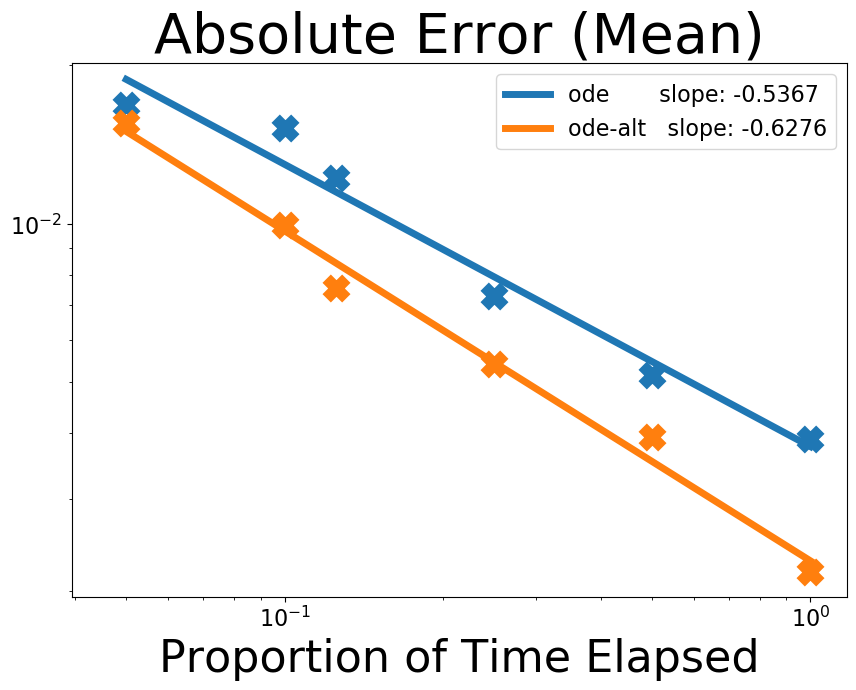
\includegraphics[width=0.475\linewidth]{figures/ode/ode_convergence_mud_obs_mean}
  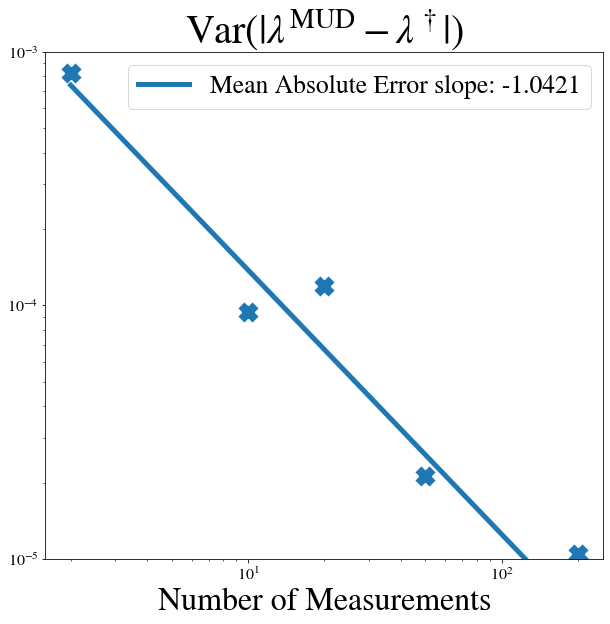
\includegraphics[width=0.475\linewidth]{figures/ode/ode_convergence_mud_obs_var}

  \caption{Convergence of the MUD point given $N=1E4$ model evaluations for increasing numbers of observations for randomly placed sensors.
  Convergence rates are estimated using first-order linear regressions in $\text{log}_{10}$-space.
  $100$Hz equipment demonstrates a reduction of uncertainty and improvement in precision as $S$ increases towards $200$.
  We observe the same rates of convergence for the alternative equipment and note the (slightly) lower overall error for equal numbers of measurements ($S=200$ corresponding to $t\in (1,2)$ in this formulation).
  }
  \label{fig:ode-convergence-obs}
\end{figure}
We sequentially incorporate $S=5, 10, 15, 20, 25, 50, 100, \text{ and } 200$ measurements and study the error in our estimate of $\param_\text{ref}$.
In the top half of Figure~\ref{fig:ode-convergence-obs}, we can observe that as more measurements are incorporated to the solution of the inverse problem, both precision and accuracy are improved.



To achieve higher precision in the estimate of the MUD point, one can use more precise measurement equipment.
Rather than a tolerance of one decimal place, we consider choices of $\tau = 0.1, 0.05, 0.01, 0.005, \text{ and } 0.001$ for $\mathbb{P}( \abs{\xi} < \tau ) = 99\%$ to select our $\sigma$ in our normal additive noise.
In Figure~\ref{fig:ode-convergence-std}, we study the absolute error's mean and variance as our measurement equipment gets more precise.


\begin{figure}[htbp]
  \centering
  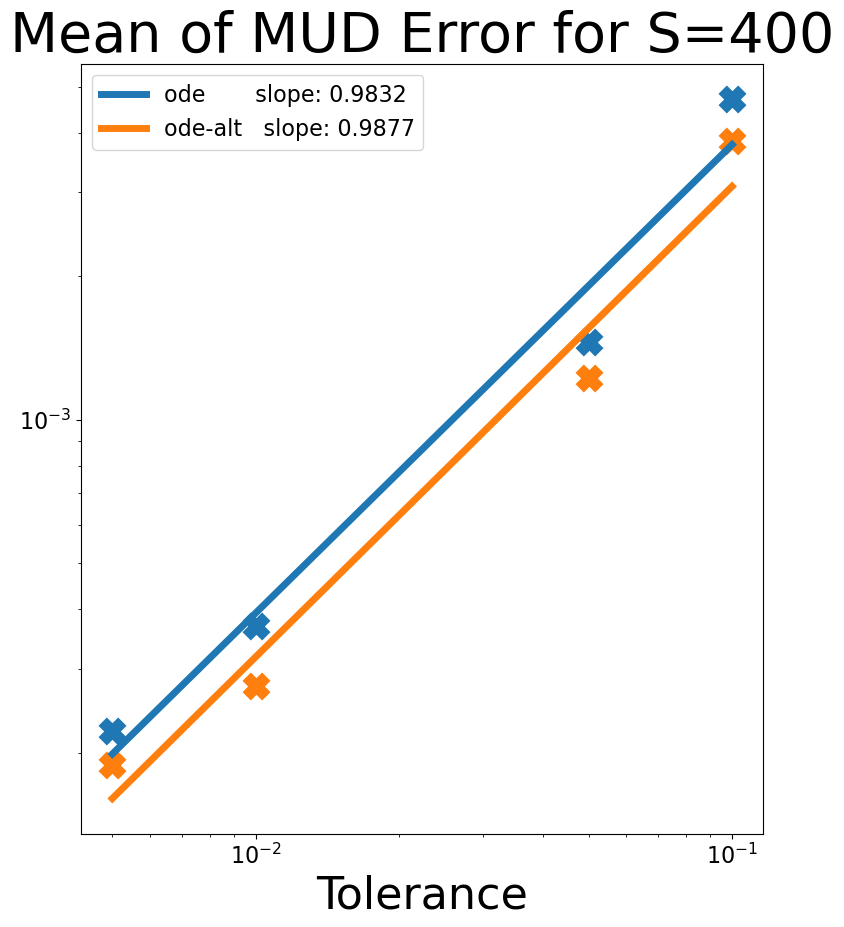
\includegraphics[width=0.475\linewidth]{figures/ode/ode_convergence_mud_std_mean}
  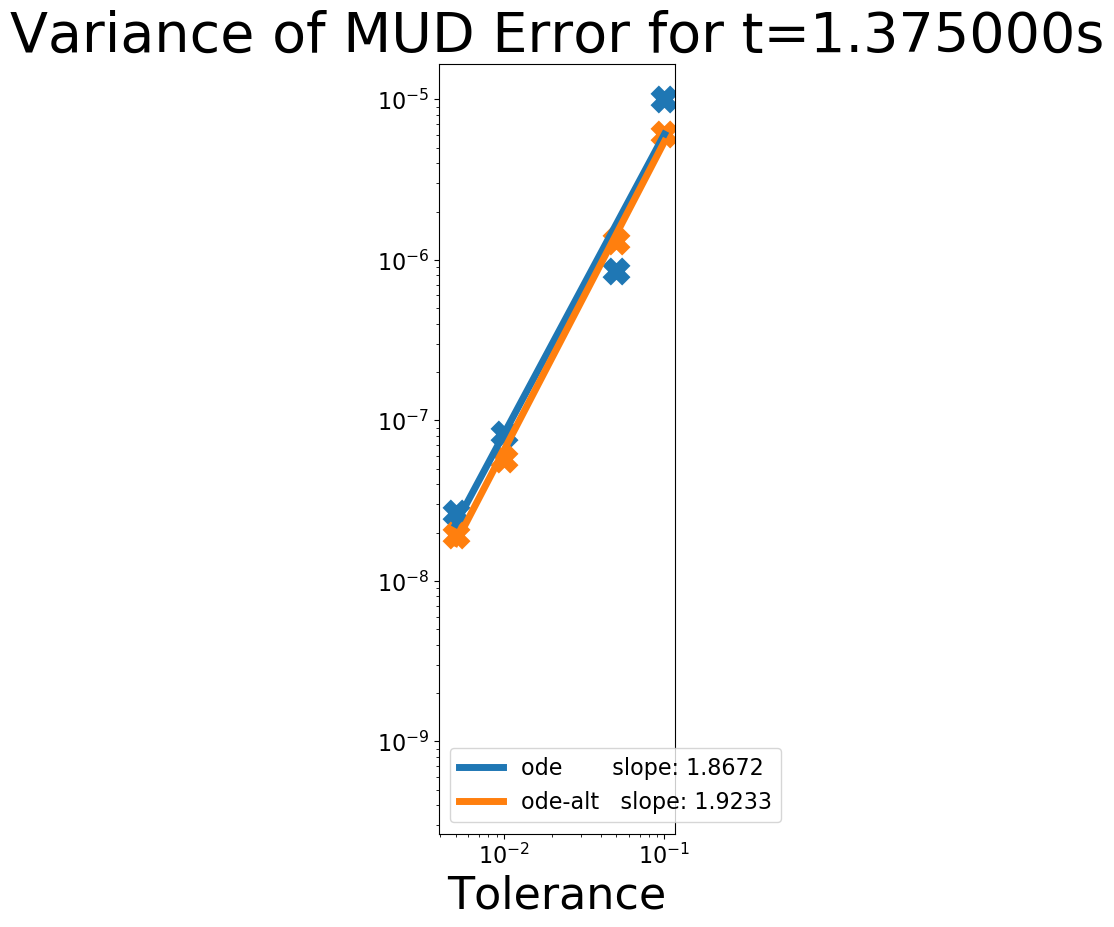
\includegraphics[width=0.475\linewidth]{figures/ode/ode_convergence_mud_std_var}

  \caption{Convergence of the MUD point given $N=1E4$ model evaluations for different precisions of observations for randomly placed sensors, incorporating $S=25$ measurements.
  As more exact measurements are incorporated, the accuracy and precision of the MUD solution improves, convergence rates are estimated with regression, and appear to be unaffected .
  }
  \label{fig:ode-convergence-std}
\end{figure}

TK - say more here.


%%%%%%%%%%%%%%%%%%%%%%%%%%%%%%%%%%%%%%%%%%%%%%%%%%%%%%%%%%%%%%%%%%%%
%%%%%%%%%%%%%%%%%%%%%%%%%%%%%%%%%%%%%%%%%%%%%%%%%%%%%%%%%%%%%%%%%%%%
\subsubsection{Different Measurement Equipment}

We consider the same problem as in the previous section to address the following question: what would happen if our measurement equipment were able to capture twice as many observations?
Instead of using equipment that operates at $100$Hz, we take $200$ measurements every second, resulting in 400 equispaced observations for $t \in (1,3)$.
All other choices involved in the experiment (assumed equipment tolerance, number of trials, parameter samples) are kept the same.

\begin{figure}[htbp]
  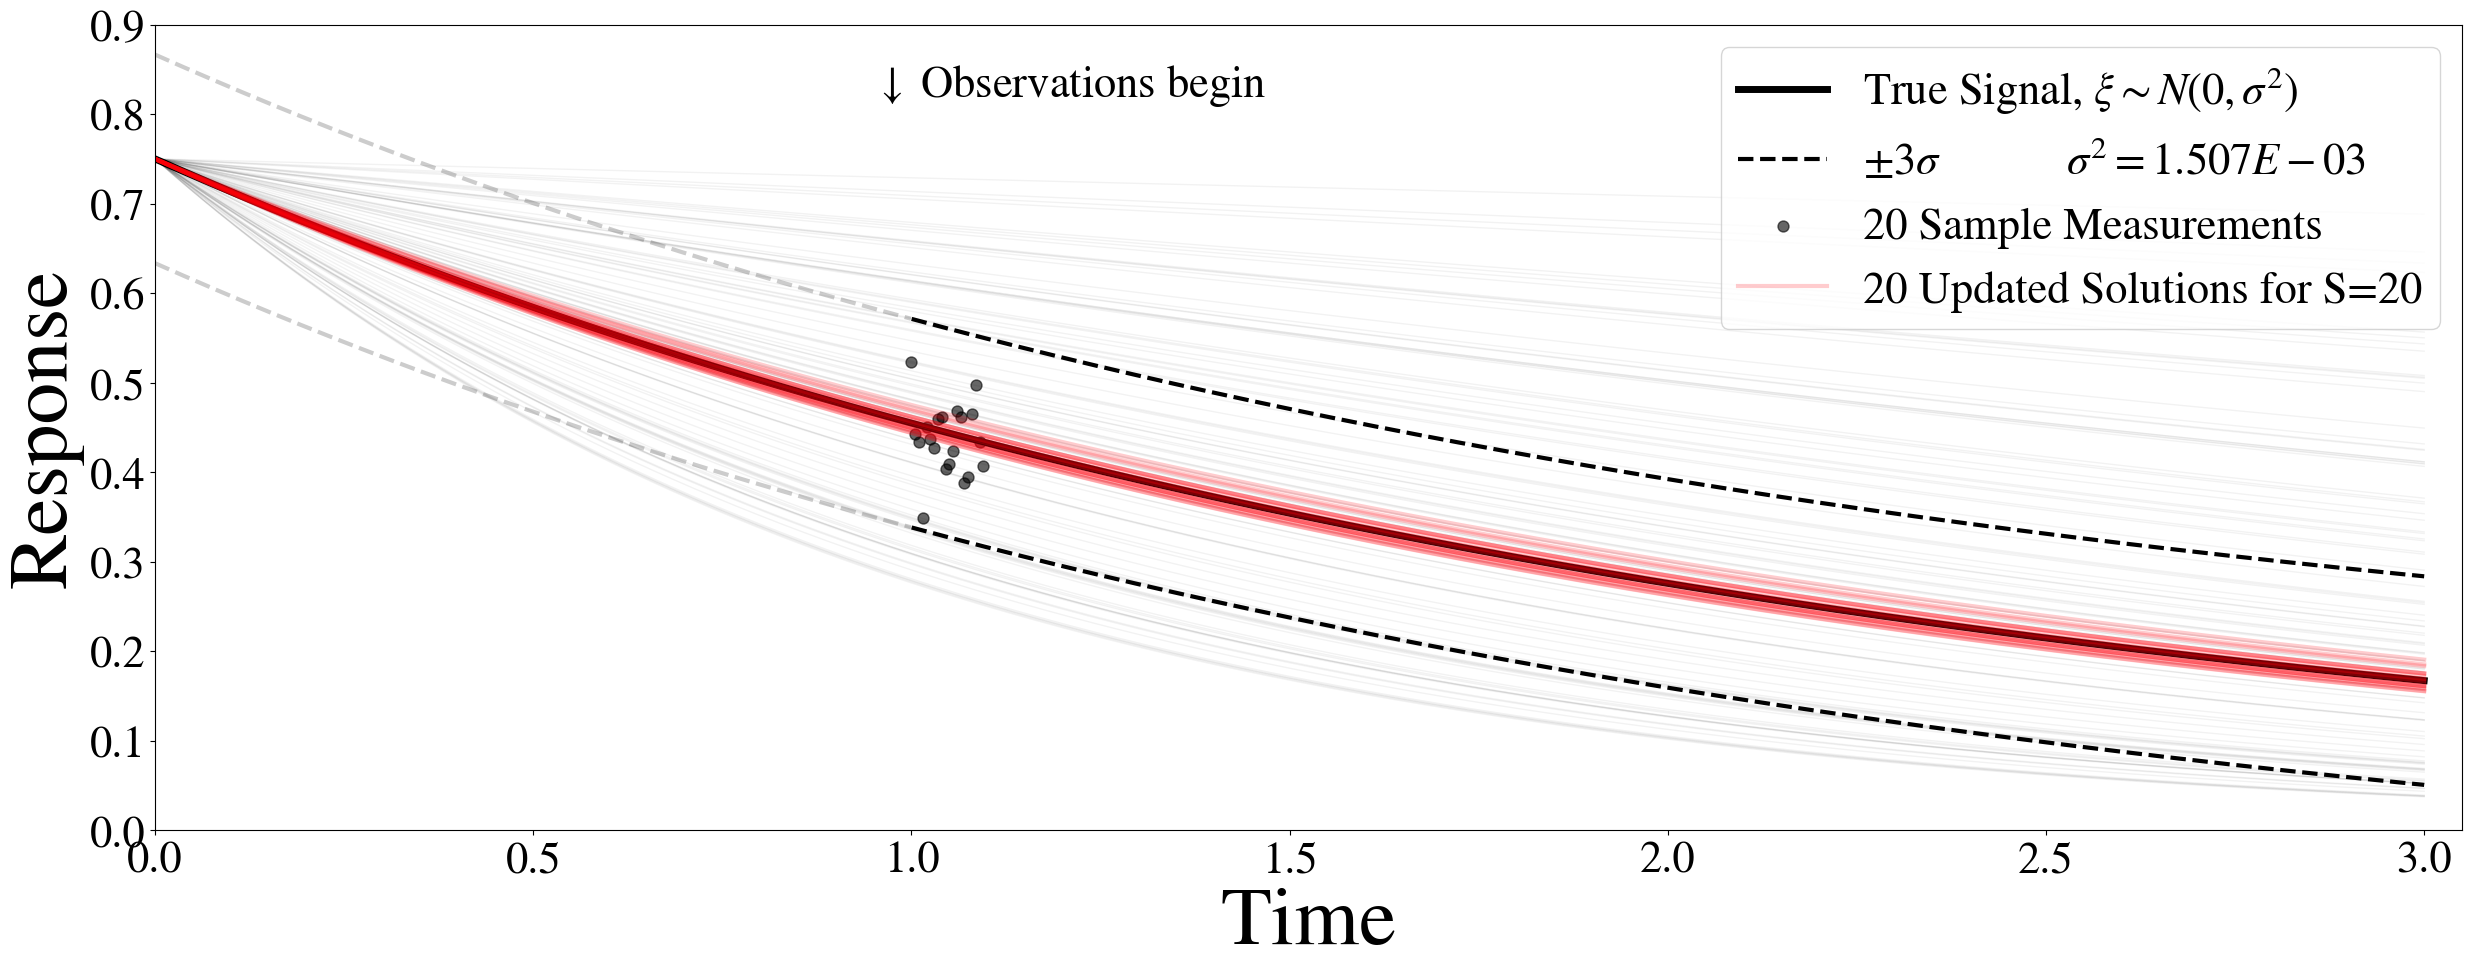
\includegraphics[width=\linewidth]{figures/ode/ode-alt_20_reference_solution}
  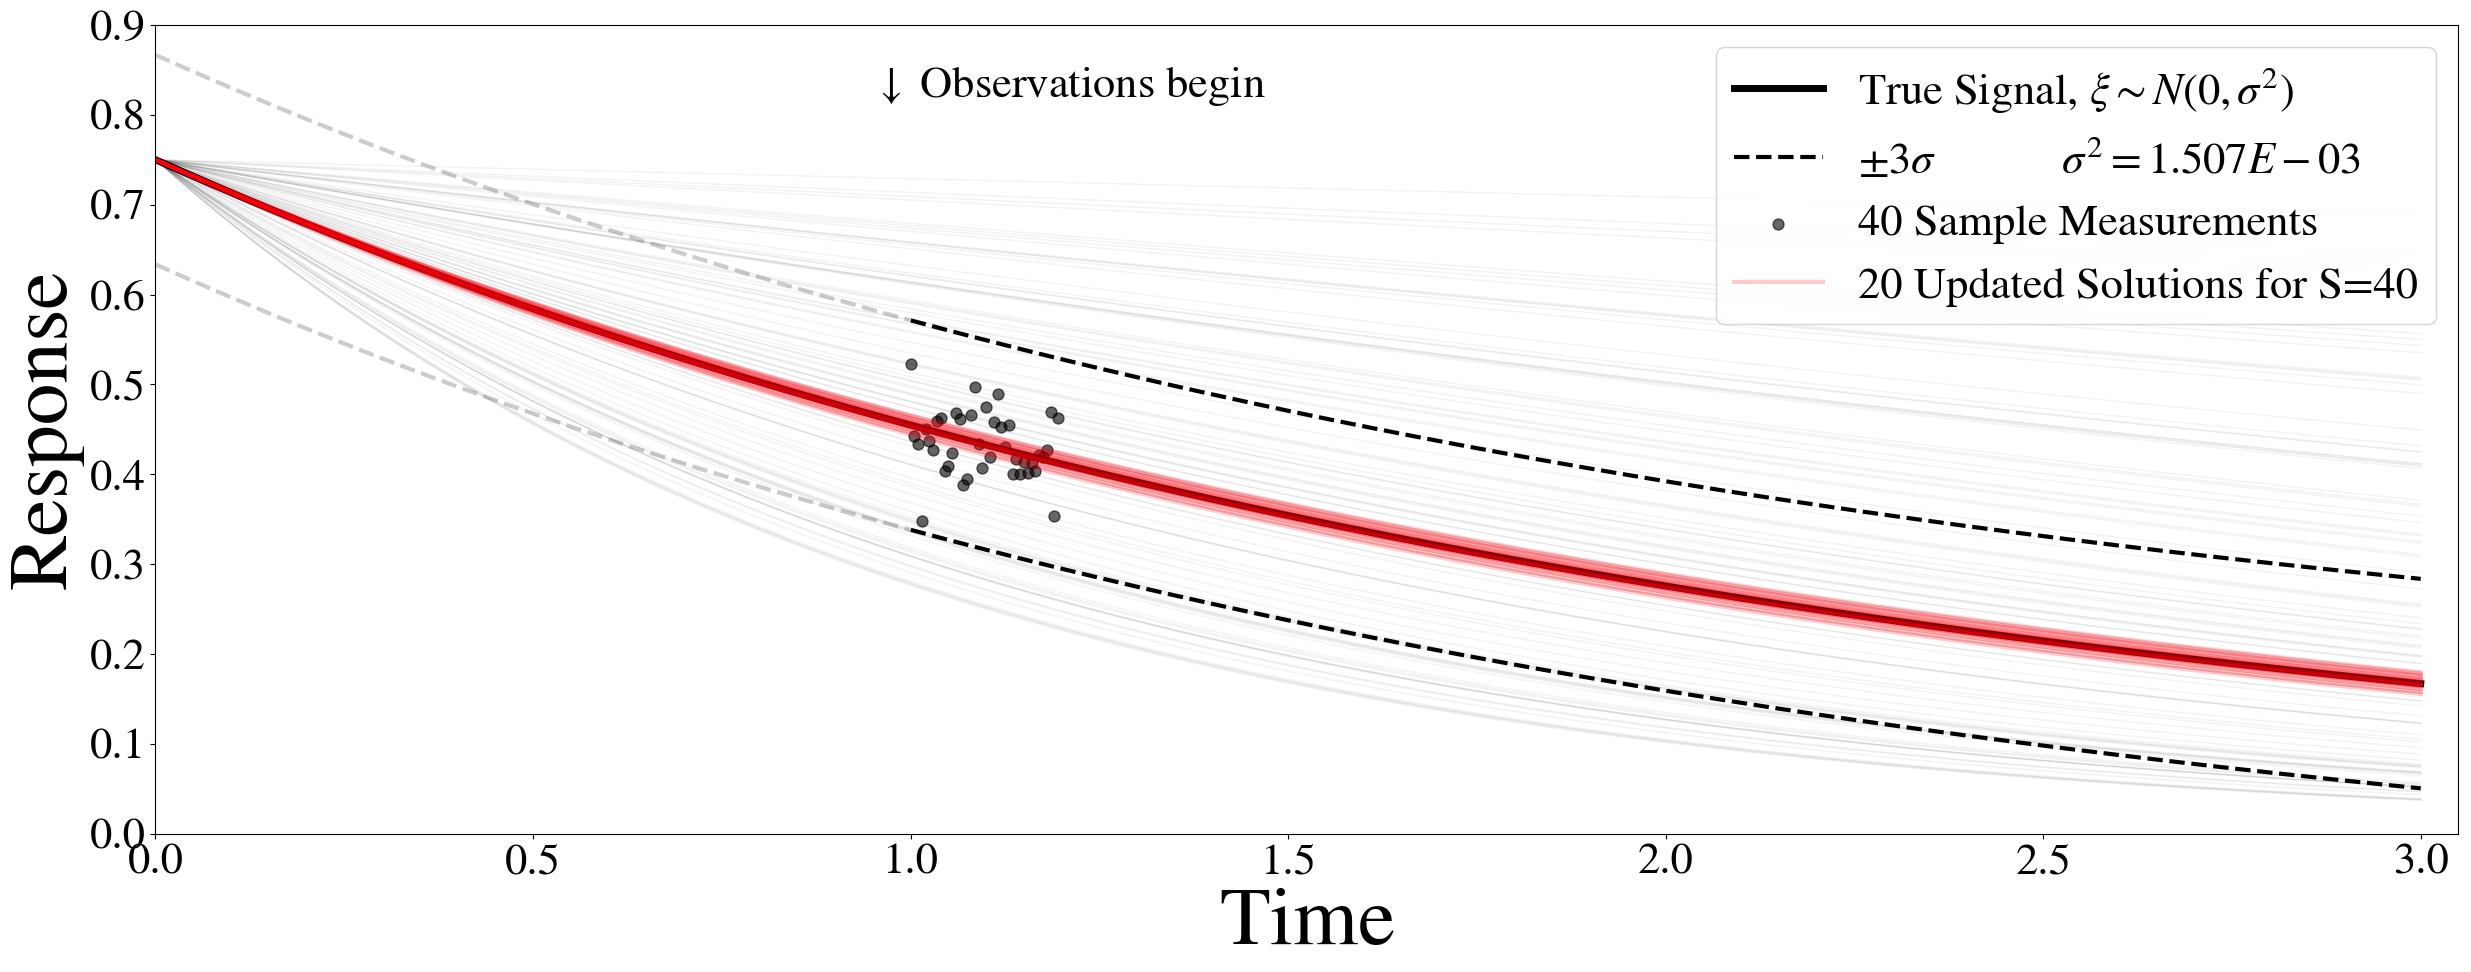
\includegraphics[width=\linewidth]{figures/ode/ode-alt_40_reference_solution}
  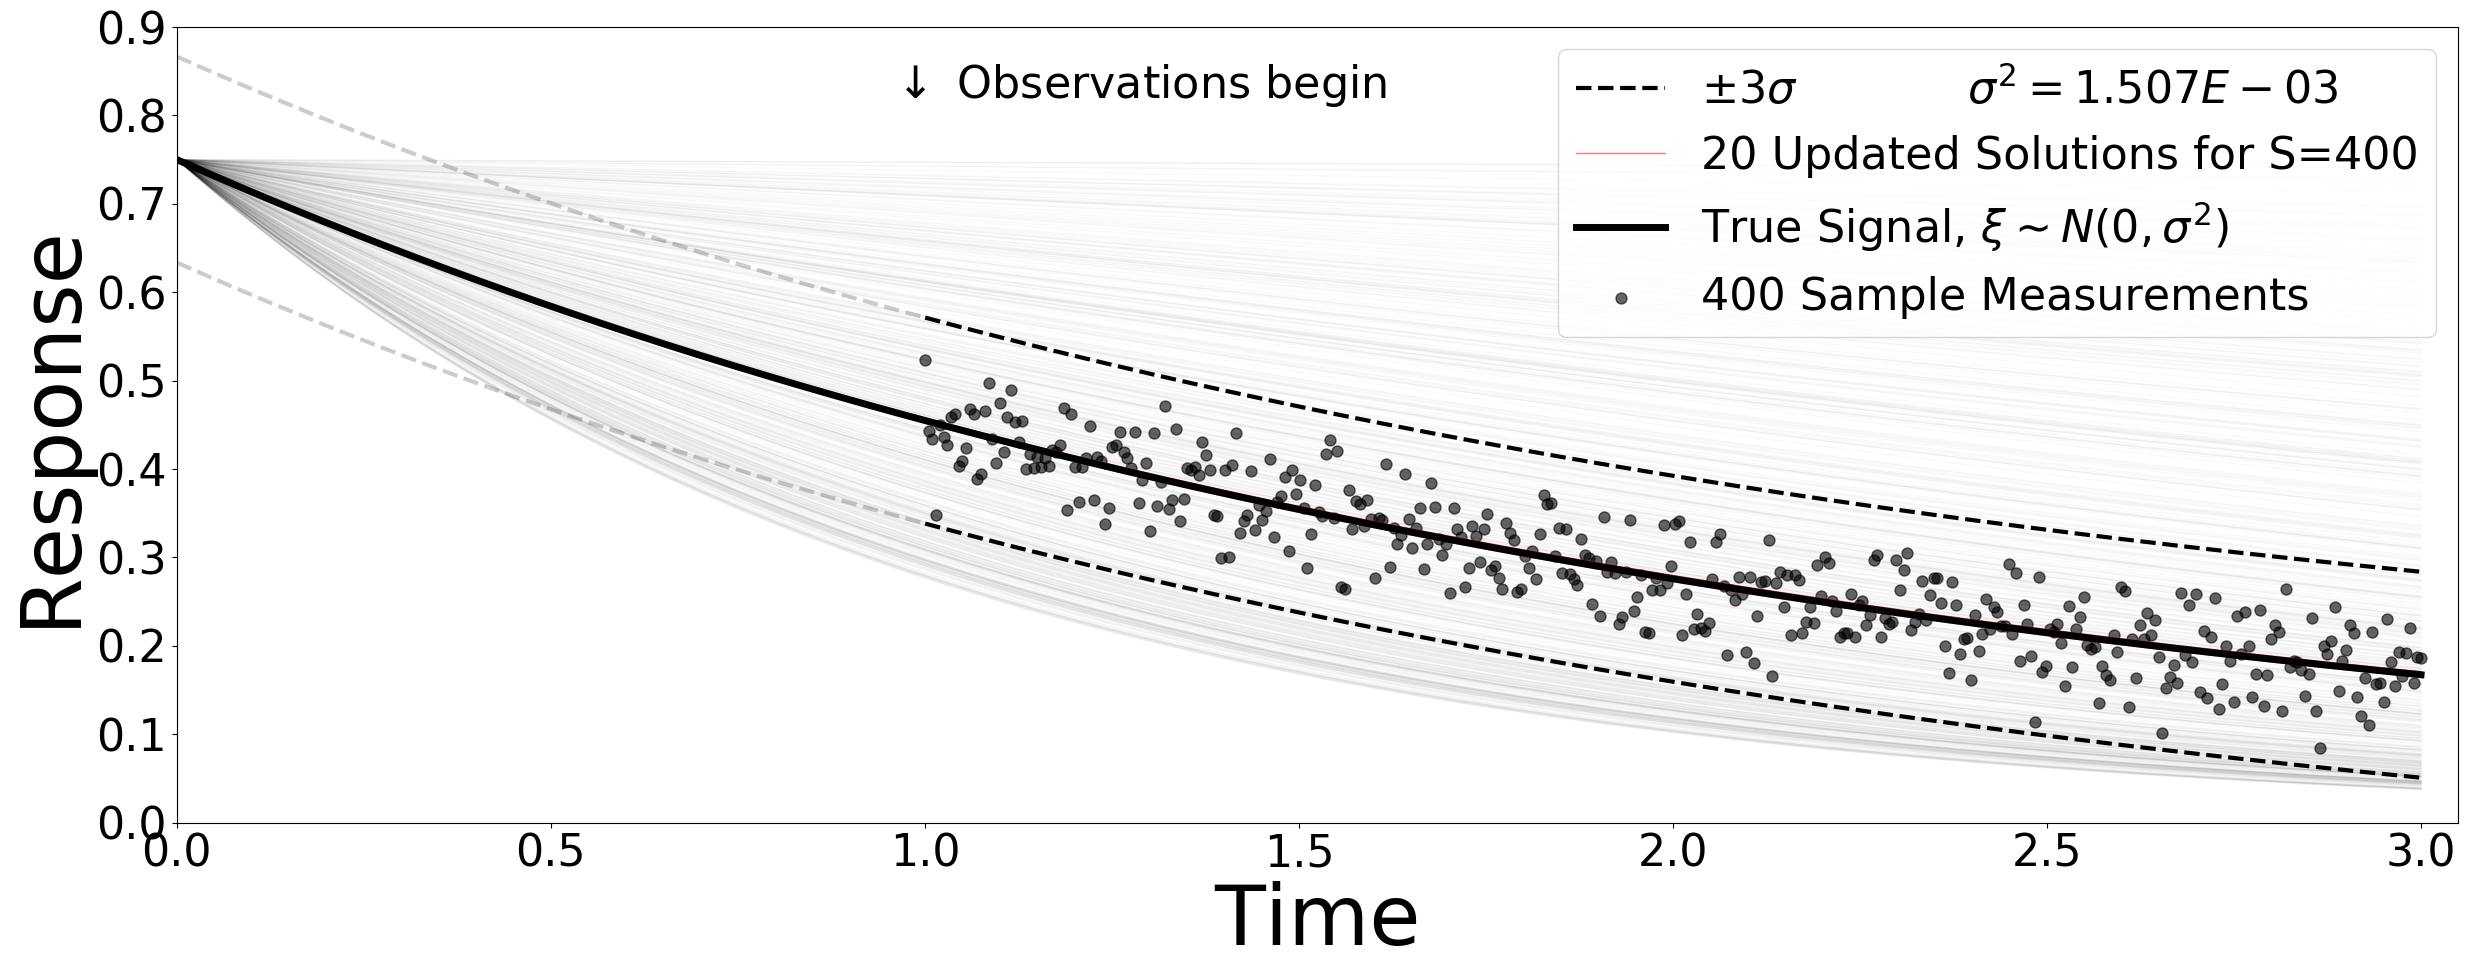
\includegraphics[width=\linewidth]{figures/ode/ode-alt_400_reference_solution}
  \caption{The associated signals for the alternative measurement equipment that operates at twice the frequency.
  The true signal is well-recovered.
  (Top): First twenty-five measurements.
  (Middle): Observations made over the same time interval as in the top half of Figure~\ref{fig:ode-reference}, corresponding to $S=50$.
  (Bottom): The entire observation window is used to solve the problem. Most of the twenty trials appear to identify the same point $\param_i$ ($1\leq i \leq N$), in the sampled parameter set.
  }
  \label{fig:ode-alt-reference}
\end{figure}
First, we note that in Figure~\ref{fig:ode-alt-reference} the predicted signals incorporating the same number of measurements look indistinguishable for $S=25$ compared to those in Figure~\ref{fig:ode-reference}.



We solve the problem for the same choices of $S$ (with the addition of $S=400$, and show the resulting error plots for convergence in the right half of Figures~\ref{fig:ode-convergence-obs} and \ref{fig:ode-convergence-std}.
The convergence rates appear to be the same and reduction in uncertainty is almost negligible.
However, we note that in the alternative setup, for an equal number of measurements, the time elapsed is half of that in the original.
This implies that we can achieve similar results with a shorter observational window by using equipment that allows for faster observations.

We have shown that the Data--Consistent approach to solving parameter identification problems manages to generalize to problems involving time-series data from a single Quantity of Interest.
We now turn our attention to an example where instead of temporal measurements, we incorporate spatial ones to solve another parameter identification problem.
% \vfill
% \pagebreak



%%%%%%%%%%%%%%%%%%%%%%%%%%%%%%%%%%%%%%%%%%%%%%%%%%%%%%%%%%%%%%%%%%%%
%%%%%%%%%%%%%%%%%%%%%%%%%%%%%%%%%%%%%%%%%%%%%%%%%%%%%%%%%%%%%%%%%%%%

%%%%%%%%%%%%%%%%%%%%%%%%%%%%%%%%%%%%%%%%%%%%%%%%%%%%%%%%%%%%%%%%%%%%
%%%%%%%%%%%%%%%%%%%%%%%%%%%%%%%%%%%%%%%%%%%%%%%%%%%%%%%%%%%%%%%%%%%%
\subsection{Elliptic PDE Example}\label{subsec:pde-example}

Consider the following Poisson problem defined on a unit domain:
\begin{equation}\label{eq:pde-equation}
\begin{cases}
\hfill -\nabla \cdot \nabla u &= f \quad\text{on } \Omega \\
\hfill u &= 0 \quad\text{ on } \Gamma_T \cup \Gamma_B \\
\hfill \frac{\partial u}{\partial \mathbf{n}} &= g(x,\param) \quad\text{ on } \Gamma_L \\
\hfill \frac{\partial u}{\partial \mathbf{n}} &= 0 \quad\text{ on } \Gamma_R
\end{cases}
\end{equation}
where $(x_1, x_2) \in \Omega = (0,1)^2$, $\Gamma_T$ is the top, $\Gamma_B$ is the bottom, $\Gamma_L$ and $\Gamma_R$ left and right, respectively.
$\frac{\partial u}{\partial \mathbf{n}}$ denotes the outward normal direction.

\begin{figure}[htbp]
\centering
  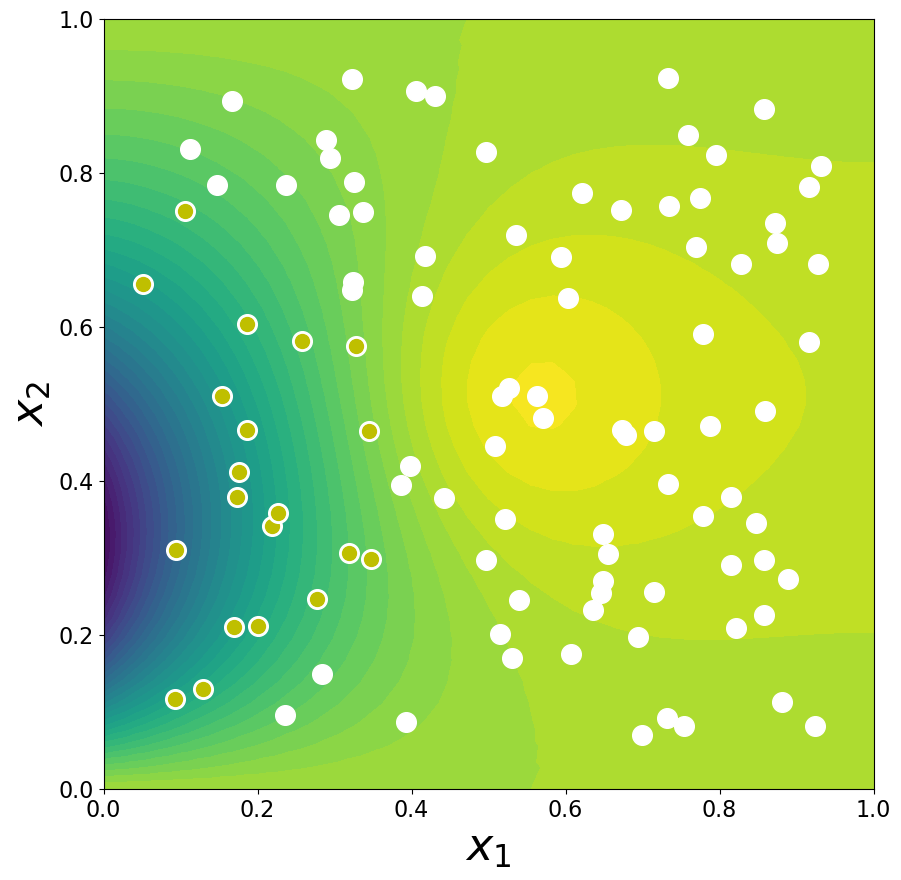
\includegraphics[width=0.475\linewidth]{figures/pde/pde_reference_solution}
  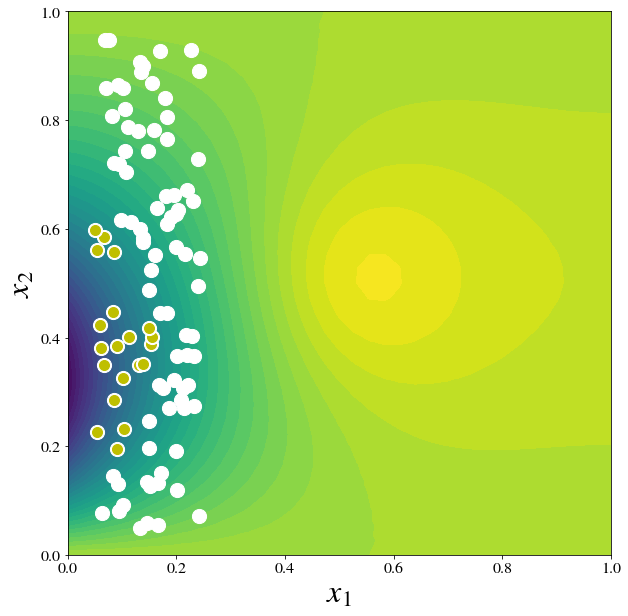
\includegraphics[width=0.475\linewidth]{figures/pde/pde-alt_reference_solution}
\caption{The function response surface for $u$ solving \eqref{eq:pde-equation} with $S=100$ measurement locations highlighted in white.
The twenty most sensitive locations are highlighted in yellow.
(Top): Uninformed sensor placement, where the most sensitive points  appear to cluster around the center of the  left boundary.
This observation is used to inform a better placement.
(Bottom): An alternative random arrangement of $S=100$ measurement locations.
}
\label{fig:pde-ref-solution}
\end{figure}
We select $g=\param \sin(\pi x_2)$, and show the response surface for our given choice of $\param = 3$ in Figure~\ref{fig:pde-ref-solution}.
Our initial density is chosen to be uniform over the interval $\Lambda = (1,5)$.
$f$ is chosen to be $10\exp\{-\frac{(x_1-0.5)^2 + (x_2 - 0.5)^2}{0.02}\}$



One could place a regular grid of sensors in the interior of $\Omega$ to simulate a sensor array of some sort.
However, observe that the response surfaces shown in Figure~\ref{fig:pde-ref-solution} exhibit vertical symmetry about the line $x_1=0.5$ (as a result of our choice of $g$).
We are interested in demonstrating the impact of incorporating more measurements, which poses a problem for this particular experimental design since it will heavily rely on the way in which the sensor grid is indexed.
For example, if the first half of indexed sensors corresponded to the bottom half of $\Omega$, the incorporation of the second half will be equivalent to having repeated observations.
Moreover, since the left-side of $\Omega$ is more sensitive to changes in $\param$ than the right, indexing in a serpentine manner will lead to sharper declines in uncertainty whenever a sensor from a different row gets incorporated.
To avoid these problems, we instead simulate the sensors as being placed randomly in the interior so that index-dependence becomes irrelevant and  probability theory ensures the lack of truly redundant measurement locations.

%%%%%%%%%%%%%%%%%%%%%%%%%%%%%%%%%%%%%%%%%%%%%%%%%%%%%%%%%%%%%%%%%%%%
%%%%%%%%%%%%%%%%%%%%%%%%%%%%%%%%%%%%%%%%%%%%%%%%%%%%%%%%%%%%%%%%%%%%
\subsubsection{Uninformed Sensor Placement}

We consider a selection of $S=1000$ measurement locations in the interior of the response surface chosen by sampling a uniform density over the set $(0.05, 0.95)^2 \subset \Omega$.
In Figure~\ref{fig:pde-sensitivity}, we plot the data generated by each simulated sensor location, and observe that some measurements are more sensitive in others.
The majority of measurements exhibit almost no sensitivity to changes in $\param$, visually represented by near-horizontal lines.
However, some of the sensors have steep slopes, indicating higher sensitivity to the unknown parameter.
To generate convergence plots, we use all thousand available measurements but solve the problem repeatedly for $S = 5, 10, 15, 20, 25, 50, 100, 250, 500, \text{ and } 1000$.


\begin{figure}[htbp]
\centering
  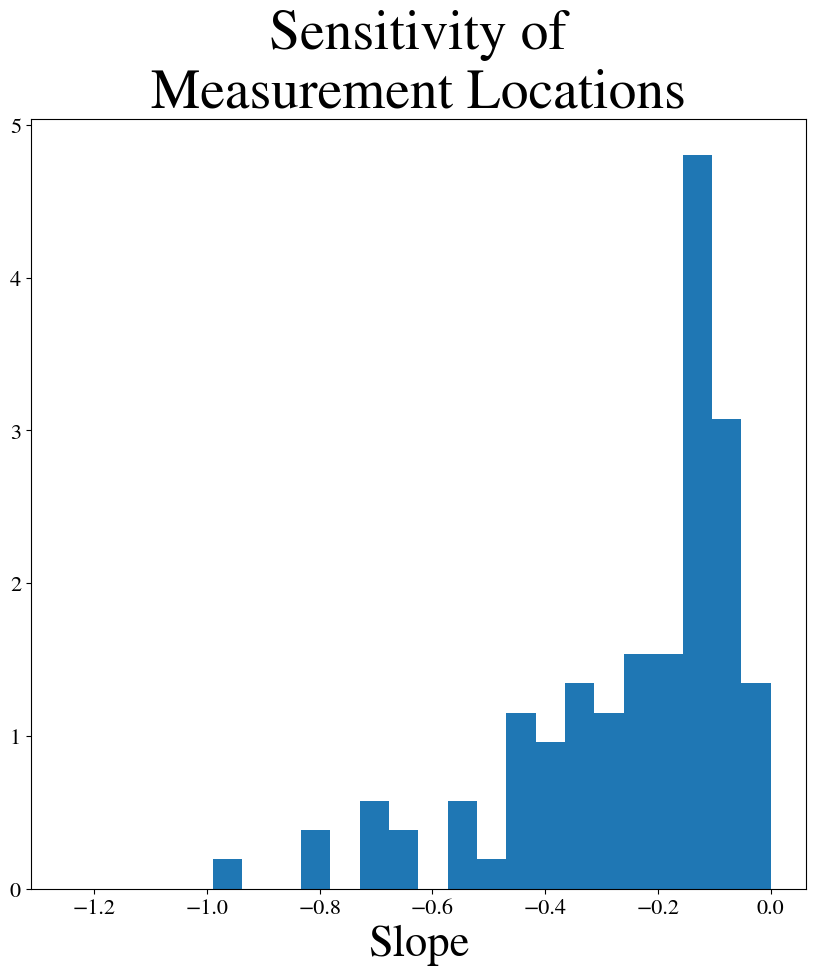
\includegraphics[width=0.35\linewidth]{figures/pde/pde_sensitivity_qoi}
  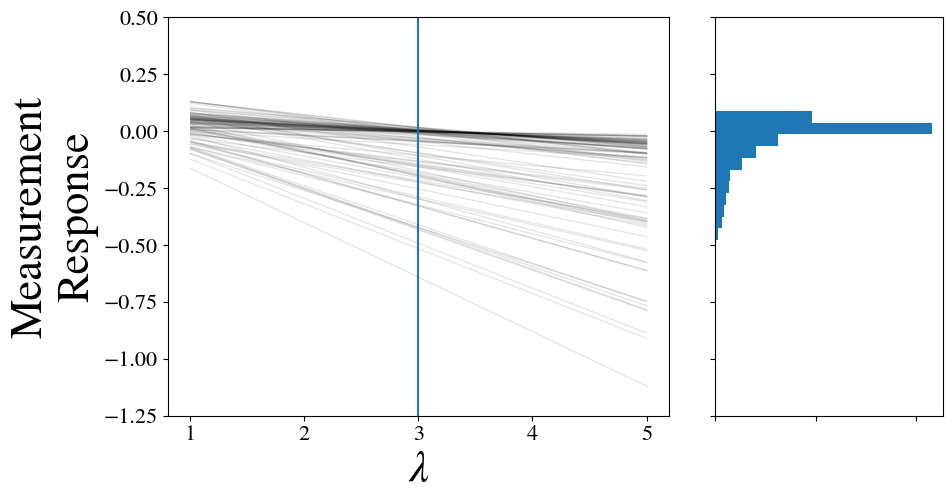
\includegraphics[width=0.6\linewidth]{figures/pde/pde_qoi_response}
  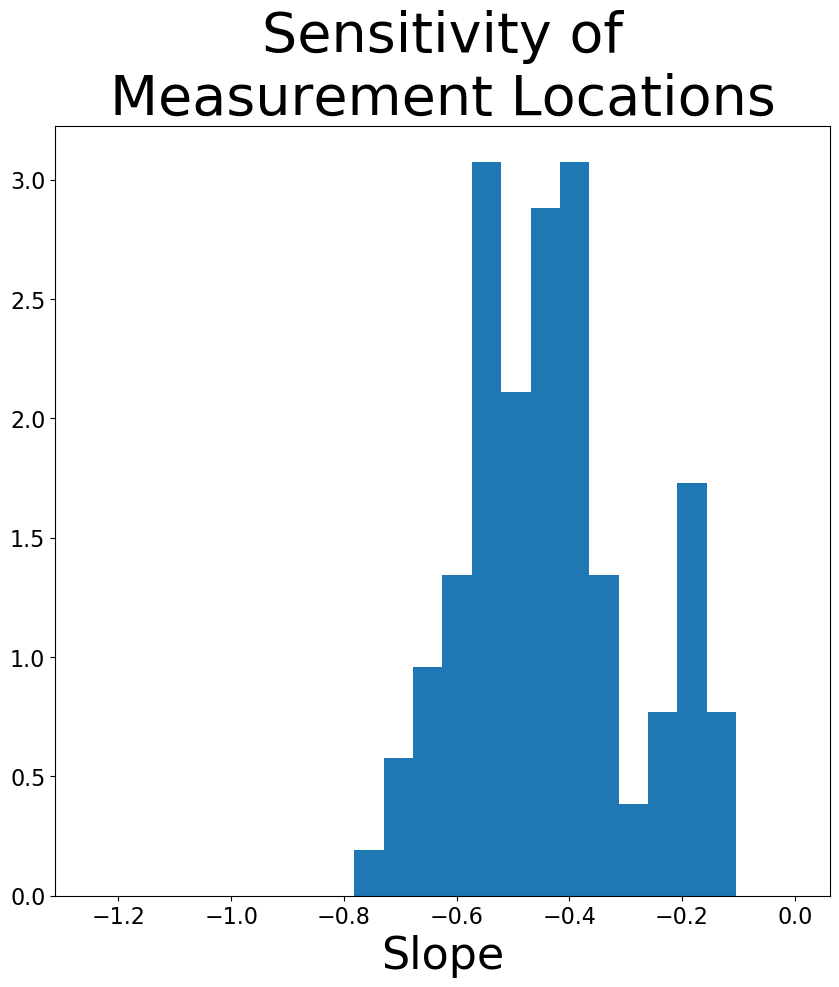
\includegraphics[width=0.35\linewidth]{figures/pde/pde-alt_sensitivity_qoi}
  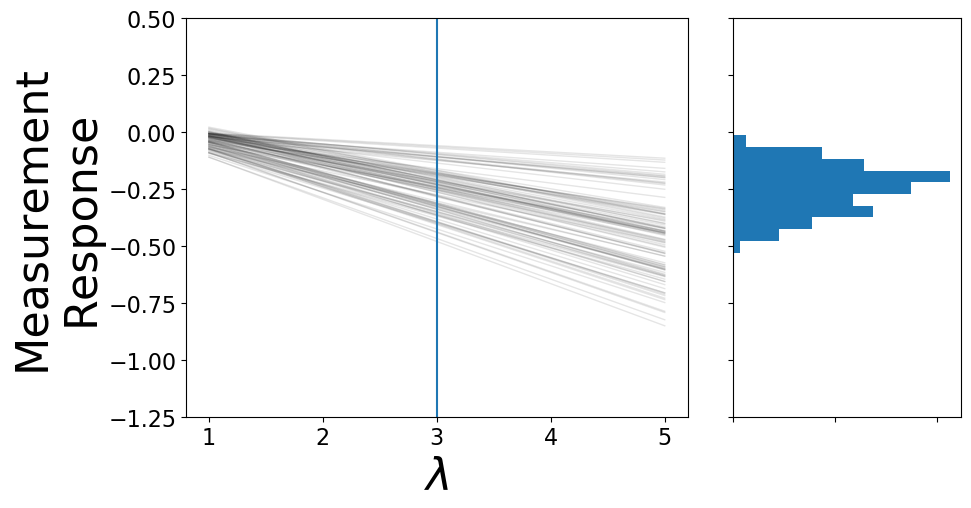
\includegraphics[width=0.6\linewidth]{figures/pde/pde-alt_qoi_response}
  \caption{We plot the values of the response surface evaluated at all $S=1000$ random measurement locations.
  The histogram depicts the measurement values of the response surface evaluated at the true parameter value $\param_\text{ref}=3$.
  (Left): Sensitivity of measurements as a function of $\param$, the scaling for the left boundary condition function.
  (Right): Since the response at each measurement location is linear with respect to $\param$, we compute the slopes for all $S=1000$ sensors and show the associated histogram.
  (Top): Uninformed sensor placement. Observe that most locations are insensitive to changes in $\param$. The ratio of most to least sensitive slopes exceeds 50.
  (Bottom): Informed sensor placement. The informed sensors have much less variability in their respective sensitivities (ratio closer to 10).
  }
\label{fig:pde-sensitivity}
\end{figure}



We are interested in knowing how the uncertainty around the parameter estimate (the MUD point) changes as we incorporate more (noisy) data.
Consider the plots in the left-half of Figure~\ref{fig:pde-convergence-obs}, which demonstrates the impact of increasing $S$ on our ability to resolve $\param_\text{ref}$.


\begin{figure}[htbp]
  \centering
  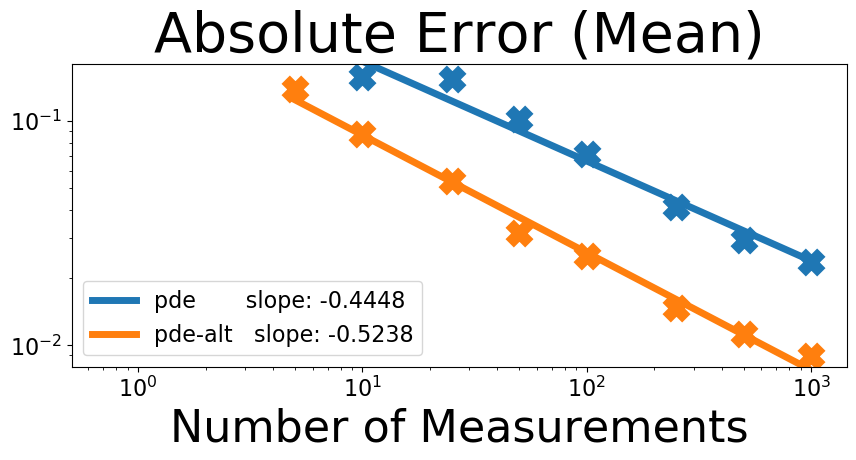
\includegraphics[width=0.475\linewidth]{figures/pde/pde_convergence_mud_obs_mean}
  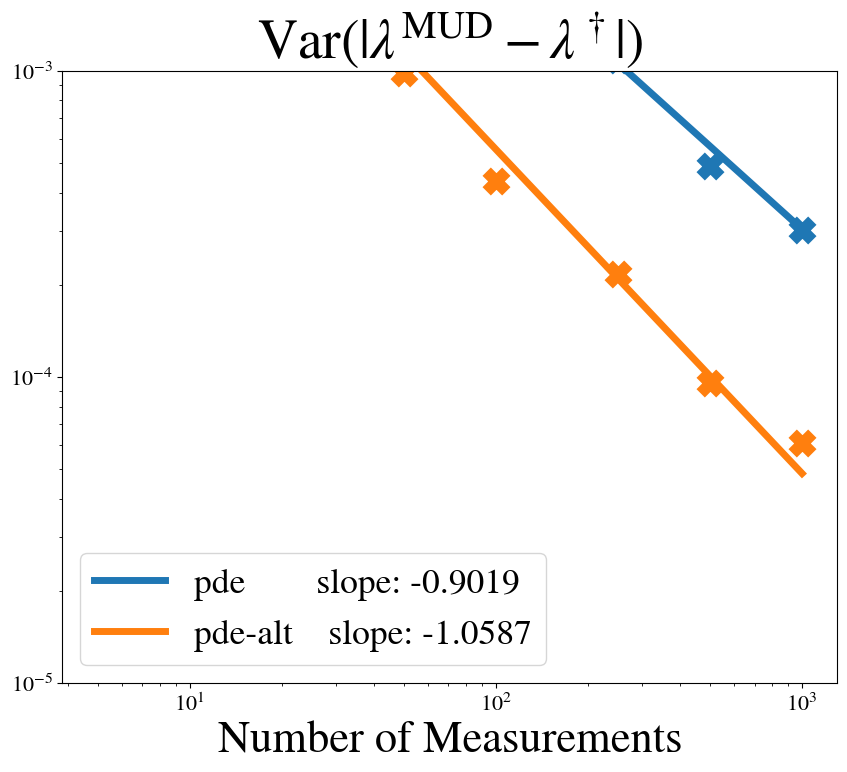
\includegraphics[width=0.475\linewidth]{figures/pde/pde_convergence_mud_obs_var}
  \caption{Convergence of the MUD point (given $N=1E4$ model evaluations) for increasing numbers of observations for randomly placed sensors.
  We observe similar rates of convergence for both arrangements of measurement locations, with a marked improvement in both accuracy and precision when an informed placement is used.
  }
  \label{fig:pde-convergence-obs}
\end{figure}


Similar to \ref{fig:ode-convergence-std}, we demonstrate that using more sensitive measurement equipment improves the estimation of the MUD point.
Again we consider choices of standard deviation associated with $\tau = 0.1, 0.05, 0.01, 0.005, \text{ and } 0.001$ for $\mathbb{P}( \abs{\xi} < \tau ) = 99\%$
In Figure~\ref{fig:pde-convergence-std}, we study the impact of more precise measurement equipment on the absolute error's mean and variance.

\begin{figure}[htbp]
  \centering
  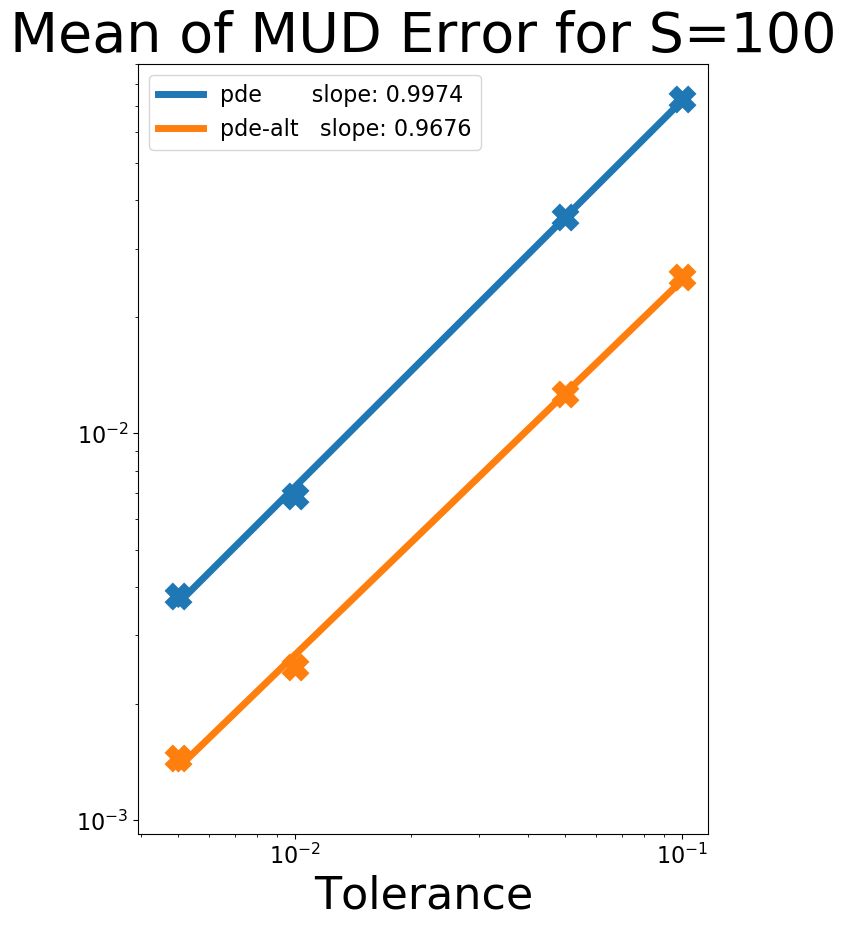
\includegraphics[width=0.475\linewidth]{figures/pde/pde_convergence_mud_std_mean}
  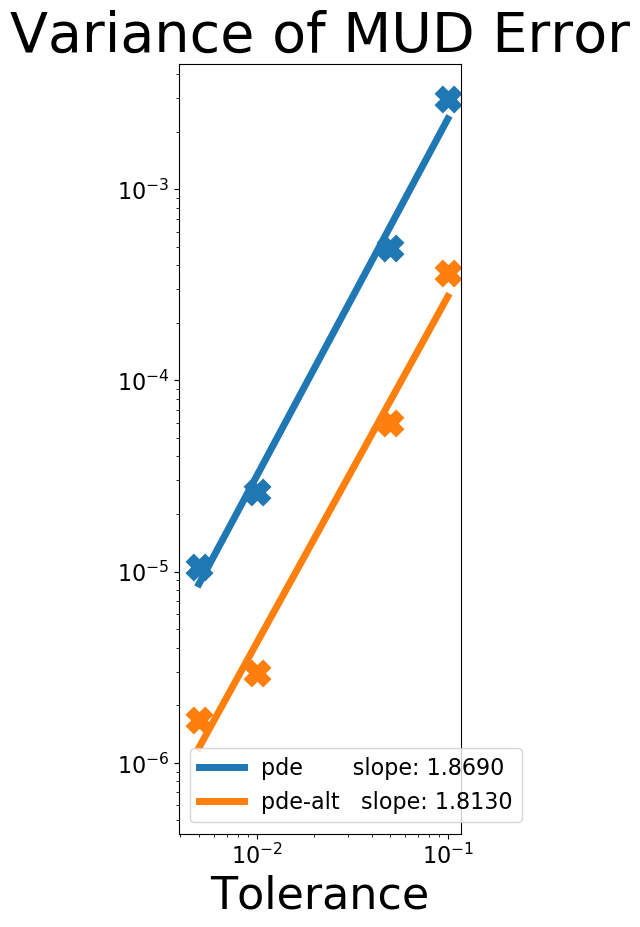
\includegraphics[width=0.475\linewidth]{figures/pde/pde_convergence_mud_std_var}
  \caption{Convergence of the MUD point given $N=1E4$ model evaluations for different measurement precisions for randomly placed sensors, incorporating $S=100$ measurements.
  We note that the convergence rates are the same but the overall accuracy and precision improve when sensors are placed in regions of $u$ that exhibit higher sensitivity to changes in $\param$.
  }
  \label{fig:pde-convergence-std}
\end{figure}


These results demonstrate that even randomly placed sensors in the interior of $\Omega$ are suitable for parameter estimation.
Figure~\ref{fig:pde-ref-solution} shows the twenty most sensitive sensors appear by the left boundary of the domain; choosing sensors more carefully using this information could lead to improved accuracy with fewer sensors.
Let us turn our attention to incroporating this observation into our experimental design chocies.

\subsubsection{Informed Sensor Placement}
Instead of placing sensors throughout the square interior of $\Omega$ given by $(0.05, 0.95)^2$, we briefly consider how the convergence results would change if the subdomain for sensors was better chosen to be near the left boundary.
Furthermore, the response surface exhibits horizontal symmetry, so we restrict locations to the bottom half of $\Omega$.
We perform the same experiment for sensors placed in $(0.05, 0.25)\times(0.05, 0.5)$ and show the results in

We demonstrate the sensitivities of each sensor in the right half of Figure~\ref{fig:pde-sensitivity}, and note that there are fewer sensors twhich exhibit low sensitivity to changes in $\param$.
It appears in the right half of Figure~\ref{fig:pde-convergence-obs}, that two decimal places of accuracy can be achieved with approximately $250$ samples instead of the $1000$ required in the left-half.


TK - Closing statements about optimal experimental design being out of the scope of this work, but how this was an interesting thing to observe.

%%%%%%%%%%%%%%%%%%%%%%%%%%%%%%%%%%%%%%%%%%%%%%%%%%%%%%%%%%%%%%%%%%%%
%%%%%%%%%%%%%%%%%%%%%%%%%%%%%%%%%%%%%%%%%%%%%%%%%%%%%%%%%%%%%%%%%%%%

%%%%%%%%%%%%%%%%%%%%%%%%%%%%%%%%%%%%%%%%%%%%%%%%%%%%%%%%%%%%%%%%%%%%
%%%%%%%%%%%%%%%%%%%%%%%%%%%%%%%%%%%%%%%%%%%%%%%%%%%%%%%%%%%%%%%%%%%%
\subsection{Concluding Remarks for Examples}

As these examples demonstrate, Data--Consistent Inversion can be used for parameter identification as a viable alternative to existing methods.
These problems have involved one-dimensional input and output spaces, and so the resulting problems were not necessarily ones that would benefit from regularization.

We point out that in the framework of collapsing available observations of data leaves the output space as scalar-valued.
As the number of parameters grows, this output dimension effectively stays fixed.
This is particularly when the DCI approach becomes advantageous.
One can incorporate a much wider variety of prior beliefs about the relative likelihoods of parameters before data is collected without compromising predictive error.
The DCI approach guarantees that the functional defined (for us, the weighted mean error) will remain accurate in spite of any encoded assumptions that are somehow at odds with data that is subsequently collected.

%%%%%%%%%%%%%%%%%%%%%%%%%%%%%%%%%%%%%%%%%%%%%%%%%%%%%%%%%%%%%%%%%%%%
%%%%%%%%%%%%%%%%%%%%%%%%%%%%%%%%%%%%%%%%%%%%%%%%%%%%%%%%%%%%%%%%%%%%

\FloatBarrier

% \
% \section{Summary of Dissertation}
%
% \
% \section{Conclusions}
%
% \
% \section{Continuity of Research}
%

\section{Miscellaneous Extensions}


\subsection{Leveraging Data in Different Ways}\label{sec:ch05-data}
Mention the other map we can use (SSE) here.

\subsection{Addressing Model Assumptions}\label{sec:ch05-variance}
Both the maps required us to have knowledge of the variance in the measurements.
What if we got it wrong?
\emph{What if we don't know the variance? How does mis-estimating it affect our solutions?}
In this section we pose some questions and provide a brief hint at a research direction but really we do not have adequate time to flesh out the answers to these, just acknowledge that they're similar concerns shared by the Bayesians.

Multiplicative noise - handled in a straightforward way, maybe put an example here and leave it at that? Put it in appendix?


\subsection{Machine-Learning Enhancements}\label{sec:ch05-ml}

Recall that in the previous chapter we demonstrated that the MUD solution retains the accuracy of least-squares solutions while simultaneously offering the flexibility of specifying initial beliefs.
Normally in order to incorporate such beliefs, practitioners in the machine-learning field would perform Tikhonov regularization, usually with the inclusion of a hyper-parameter which scales the additional parameter-space norm in the objective function.
Mathematically, this scaling factor applied to the norm is equivalent to scaling the matrix representation of the initial (prior) covariance.
Increasing this scaling factor is interpreted as having less confidence in these initial assumptions.
Conversely, decreasing it is equivalent to putting more emphasis on the prior beliefs than the evidence provided by the data, which causes MAP solutions to drift away from the solution contour (equivalence class) to which $\paramref$ belongs.

We summarize again that the MUD point is not impacted by such a scaling of the initial covariance, providing \emph{consistent} solutions which demonstrate levels of accuracy that MAP points only exhibit for larger values of scaling factors.
Not only is it robust to the specification of prior assumptions, but it manages to offer the flexibility of such specifications without paying the additional cost of hyper-parameter optimization that would be required for the Tikhonov solution to achieve comparable results; any choice of $\alpha$ would have sufficed.

By contrast, the Tikhonov-regularized solution selects a point that is biased in directions defined by the initial density (covariance).
The observation-consistent solution is an update to the initial mean in this same direction but always lies on the contour $Q^{-1}(\observedMean)$.
The trouble is, none of these regularization approaches actually guarantee that in under-determined problems, the unique solutions that are selected are close to $\paramref$.

We show that regardless of how well-informed your beliefs are, the convergence rate of the MUD solutions as more data is incorporated\---either by dimension or rank)\---will match those of the Least-Squares solutions.
Moreover, unlike MAP solutions, the MUD point is not sensitive to scaling of the initial covariance (how strongly initial beliefs are held).
This insensitivity provides a strong motivating factor for the consideration of the observation-consistent approach within the standard set of solution methods available to scientists and modelers who seek to perform parameter-identification.
We leave the investigation of more connections to the removal of hyper-parameter estimation to future work.

[TK - can put example here about MCMC extensions, sequence of problems with resampling from updated densities. Have a notebook's worth of results with the Rosenbrock]


\section{Sequential Inversion}\label{sec:ch05-sequential}

The DCI framework relies on evaluating the ration function $r(\param)$ in $\dimD$--dimensional QoI space, so we turn our attention to addressing the challenges associated with the growth of this space.
As $\dimD$ increases, we must approximate a push-forward distribution with perhaps a fixed number of samples (from model evaluations) $\nsamps$, which represents a considerable source of error since the convergence rate for kernel density estimation with Gaussian kernels is $\mathcal{O} (N^{2+\dimD})$.

For example, suppose we have a time-dependent problem for which hundreds of spatial sensors are providing streams of data.
Approximating a hundred-dimensional space with $\nsamps = 1E3$ or $1E4$ samples (as we have been using for demonstrations), is wrought with problems.
However, either of these values for $\nsamps$ would be sufficient to estimate a one-dimensional distribution.
In some sense, approximating a QoI at each location over time is reasonable, but doing so for all of them simultaneously is not.
To this end, we propose to investigate an approach to solving the parameter estimation problem by performing inversion through a sequence of scalar-valued QoIs rather than employ a vector-valued approach.

We could choose any dimension below $\dimD$, but this sequential-scalar-valued approach provides a starting place and admits a simplicity in exposition.
By choosing a dimension of 1, we can focus solely on the order in which QoIs are inverted and dismiss the additional complexity of enumerating the combinations of QoI when dimensions can vary.
We also choose to use a linear map for convenience so that we can use the analytical solutions presented in the previous chapter without concern for approximation error.

With each iteration in the sequence of inverse problems, we are in-effect trying to explain measurements that constitute a single QoI at the expense of accuracy in others.
By contrast, the vector-valued approach seeks accuracy in all of the simultaneously.
This trade off is all about convenience, since 1-dimensional problems are computationally ``cheap,'' we can iterate through many more of them for the same computational cost.
Since by the time we finish iterating through all available QoI, the error in $Q^{(1)}$ may have been allowed to drift quite significantly away from its solution contour through the sequence of inverting through $Q^{(1)}, Q^{(2)}, \dots Q^{(100)}$.
To address this, we perform multiple passes through our set of QoI.
Borrowing from other sequential algorithms, these ``epochs'' will allow us to iterate until the solution stops changing by some predefined relative threshold, representing a lack of ``learning'' through continued effort.

We study the following motivating two-dimensional example with QoI defined by ten equispaced rotations of the unit vector $[0, 1]$ through the first two Euclidean quadrants.
We first plot the result of a single epoch in Fig.~\ref{fig:iterative-linear-demo}
\begin{figure}
  \centering
  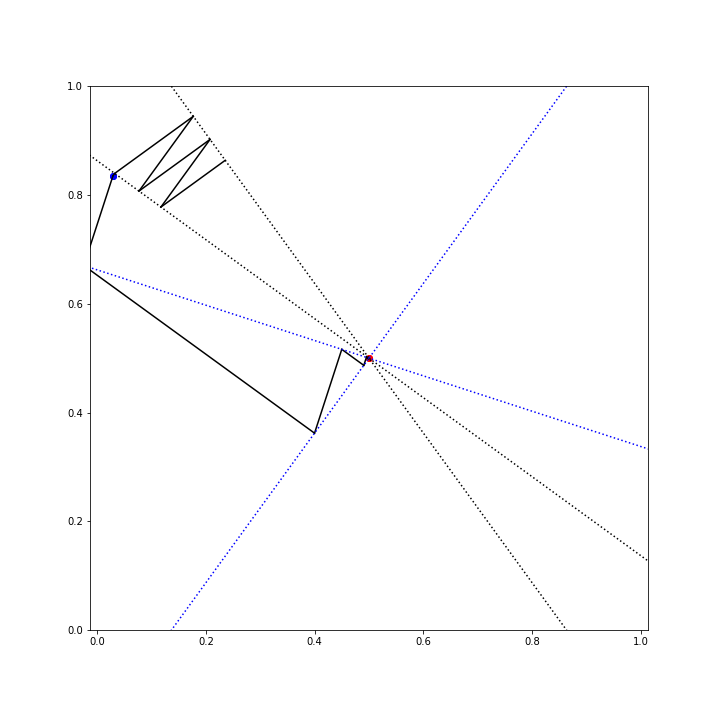
\includegraphics[width=0.475\linewidth]{examples/iterative/10D-firstepoch}
  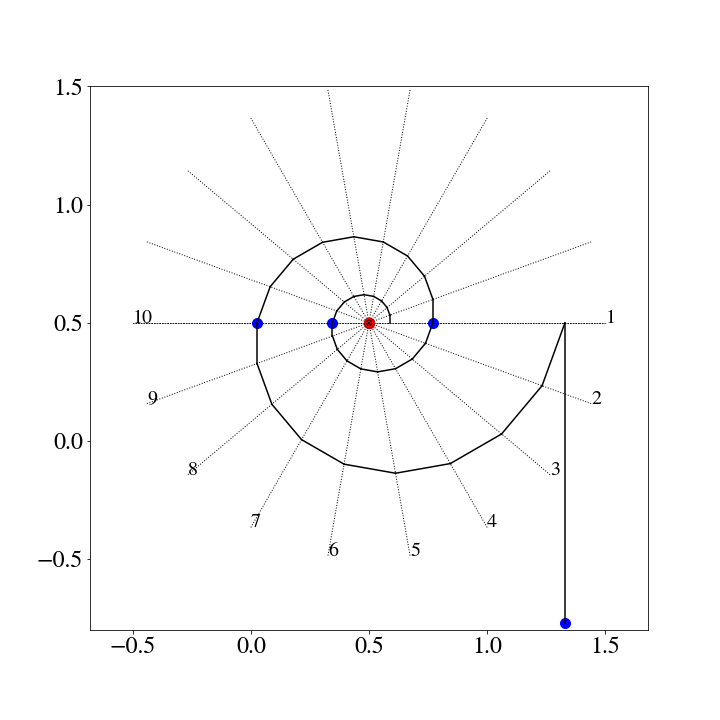
\includegraphics[width=0.475\linewidth]{examples/iterative/10D-fewepochs}

  \caption{
  Dotted lines show the solution contours for each row of the operator $A$.
  (Left): First epoch for iterating through 10 QoI.
  (Right): Three more epochs allows our estimate to get much closer to the true value.
  }
  \label{fig:iterative-linear-demo}
\end{figure}

The spiral shape is a result of the underlying geometry of this QoI map defined by rotations. The successive rows are so similar to each other that very little is ``learned'' between each iteration; the projection doesn't cover a large distance in $\pspace$.
To drive this point home, we choose two pairs of indices from among the ten available in order to define two QoI maps, the contours for which we plot in different colors in Fig.~\ref{fig:iterative-linear-demo-pair}.
We solve a total of ten 1-D inverse problems for each of them (five epochs) to match the budget of the previous example (with ten maps and one epoch).

\begin{figure}
  \centering
  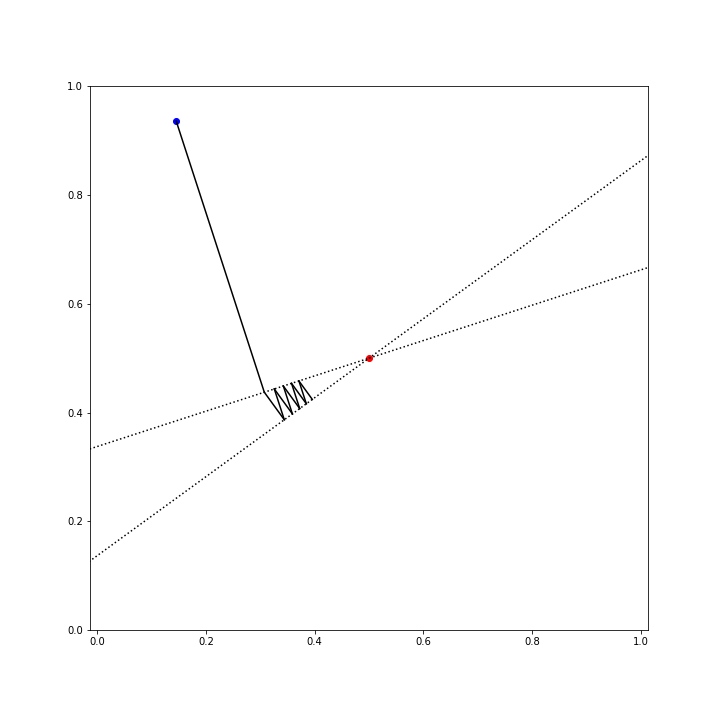
\includegraphics[width=0.475\linewidth]{examples/iterative/10D-fewepochs-pair}
  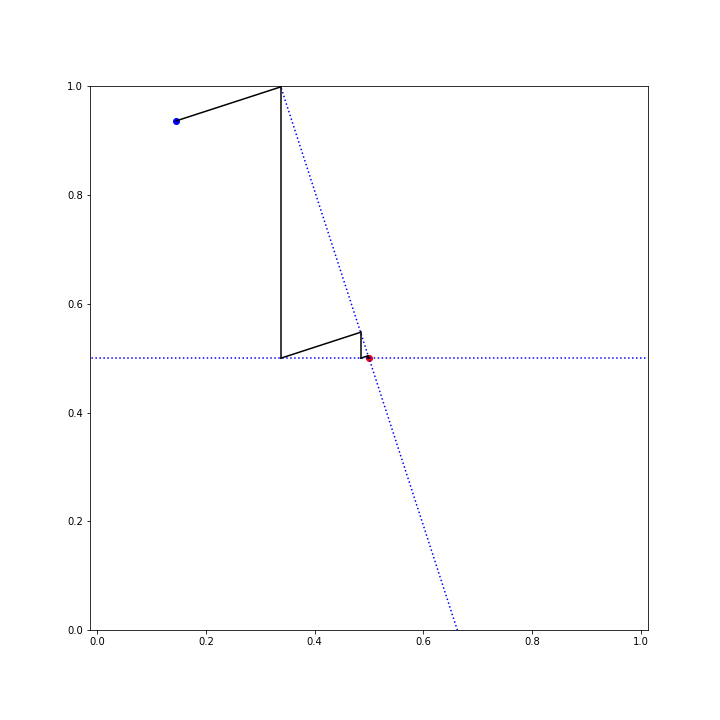
\includegraphics[width=0.475\linewidth]{examples/iterative/10D-fewepochs-pair-alt}
  \caption{
  Iterating through five epochs of two QoI, each formed by picking two of the ten available rows of $A$ at random.
  }
  \label{fig:iterative-linear-demo-pair}
\end{figure}

We observe that in Fig~\ref{fig:iterative-linear-demo-pair}, we are able to achieve much greater accuracy in estimating the true parameter value than in the case of Fig~\ref{fig:iterative-linear-demo}.
The reason for this difference is that there is more mutually distinct information between successive iterations of a pair of random rows of $A$ than there is between adjacent rows, as measured by the angle between the solution contours.

\begin{figure}
  \centering
  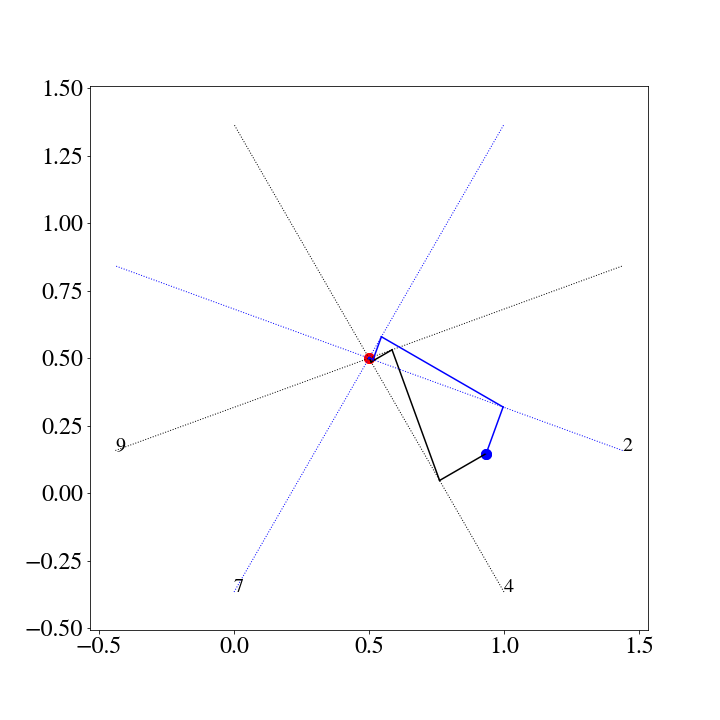
\includegraphics[width=0.475\linewidth]{examples/iterative/10D-firstepoch-pair-smart}
  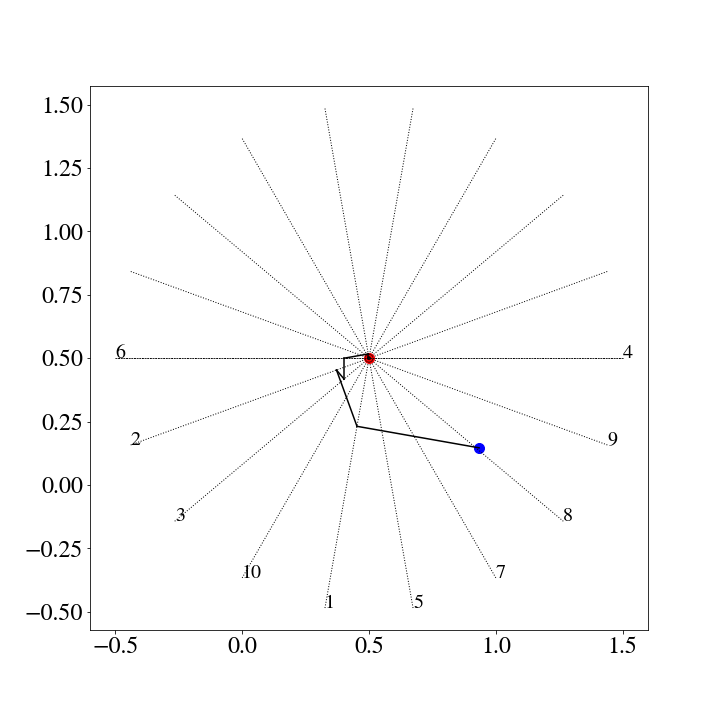
\includegraphics[width=0.475\linewidth]{examples/iterative/10D-firstepoch-rand}
  \caption{
  If we are careful with how we construct our maps or choose our iteration strategy, we can achieve considerably more accurate solutions with the same computational cost.
  (Left): Iterating through a single epoch with a QoI formed by picking rows of $A$ which exhibit mutual orthogonality.
  (Right): Iterating through the rows of $A$ at a random order for a single epoch results in considerably more accuracy than doing so in the original order of rows of $A$.
  }
  \label{fig:iterative-linear-demo-smart}
\end{figure}

Had we chosen a pair of rows that were orthogonal, the initial mean would converge to the reference value in a single epoch (two iterations), since there is no redundancy in information whatsoever.
We show this in the left half of Figure~\ref{fig:iterative-linear-demo-smart} for two orthogonal pairs.
If we instead choose to perform no a-priori analysis of the rows of $A$ and iterated through them at random, we actually also manage to accomplish a lot more accuracy for the same amount of iterations, as seen in the right half of the figure.


\subsection{Comparisons and Convergence Results}

To make these results more concrete, we propose the following example:
We limit ourselves to solving 100 inverse problems (i.e. up to ten epochs for this map), with the \emph{only} difference between approaches being the order in which the rows of $A$ are used.
First, we use the QoI as they are presented to us, in order with respect to increased rotation angle (which defines the rows of $A$).
Next, we shuffle the rows and then perform ten epochs.
Lastly, we create an ordering based on a random shuffling of the indices representing the rows of $A$, repeated ten times, for which only a single epoch is performed.
The latter approach is similar to the second in that the same problems are solved the same number of times overall, but it lifts the restriction that a row must only be used once in each effective ``epoch''.

\begin{figure}
  \centering
  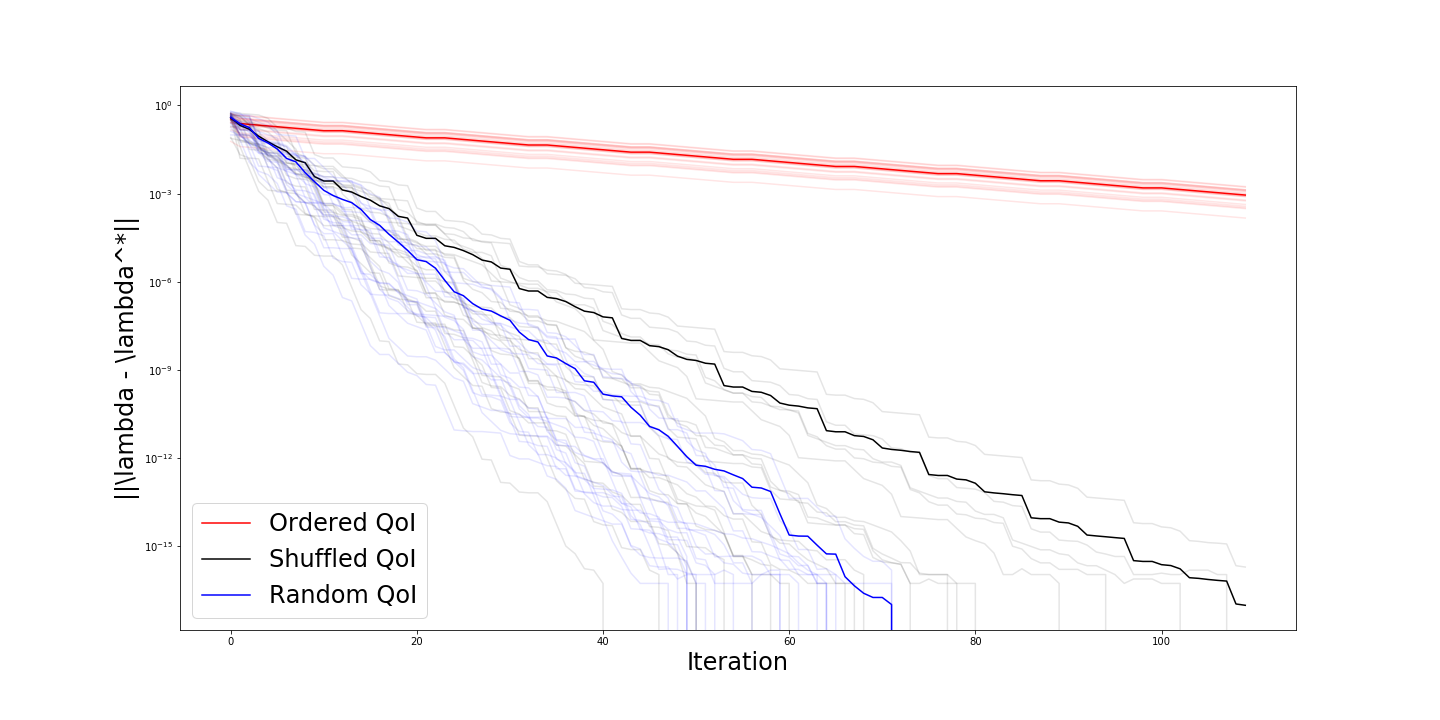
\includegraphics[width=0.95\linewidth]{examples/iterative/10D-convergence-comparison}
  \caption{
  Twenty different initial means are chosen and iterated on for three approaches.
  Individual experiments are transparent and the mean error is shown as solid lines.
  In the \emph{Ordered} approach, we iterate through the rows of $A$ as they are given to us for ten epochs.
  \emph{Shuffled QoI} refers to establishing a different random ordering of the rows of $A$ for each trial, and then
  using this ordering for ten epochs.
  Finally, in the \emph{Random QoI} approach, we choose a QoI at random for each of 100 iterations, where the ordering still ensures each row gets used ten times, representing the same overall set of inverse problems solved as the other two.
  }
  \label{fig:iterative-convergence-comparison}
\end{figure}

We see in Figure~\ref{fig:iterative-convergence-comparison} that using the rows of $A$ sequentially performs very poor, which aligns with ``spiraling'' seen in Figure~\ref{fig:iterative-linear-demo} where the first few epochs were plotted.
Shuffling the rows but requiring that every tenth iteration to use the same row (i.e., ensure same ordering for each epoch), leads to a considerable improvement by which sixteen decimal places of accuracy are achieved in under $100$ iterations.
In a few instances, the shuffled approach stumbles on an ordering that accelerates convergence, likely due to orthogonal pairs of rows in the shuffled order.
These cases exhibit the kind of behavior we saw in the left panel of Fig~\ref{fig:iterative-linear-demo-smart}; in other words, sometimes our random shuffling finds the ``smart'' rows to iterate through.
Since the ordering has no dependence on iteration number in the approach where we use random rows, we have more opportunities to find these successive orthogonal pairings, and so we see that on average, it takes fewer iterations to achieve the same accuracy.


\subsection{Iterated Solutions for a PDE Example}\label{sec:iterated-nonlinear}

Batch-updates is the connection to make here.
We are going to set up the heatrod example here but place measurement devices throughout and record the measurements at several intervals in time, the point being here that the dimension of the QoI will be higher than the input space but it's okay because we're iterating.

Some systems will be more informative early in time, others late, so the best thing to do is not really something we're going to answer, we're just going to show how this approach \emph{could} work in a situation like this where the data is streaming in over time.

\FloatBarrier
